\documentclass[border=10pt]{standalone}

\usepackage{tikz}
\usepackage{tikzsymbols}
\usetikzlibrary{calc,patterns,shapes.geometric}

\def\centerarc[#1](#2)(#3:#4:#5){\draw[#1] ($(#2)+({#5*cos(#3)},{#5*sin(#3)})$) arc (#3:#4:#5);}

\begin{document}
	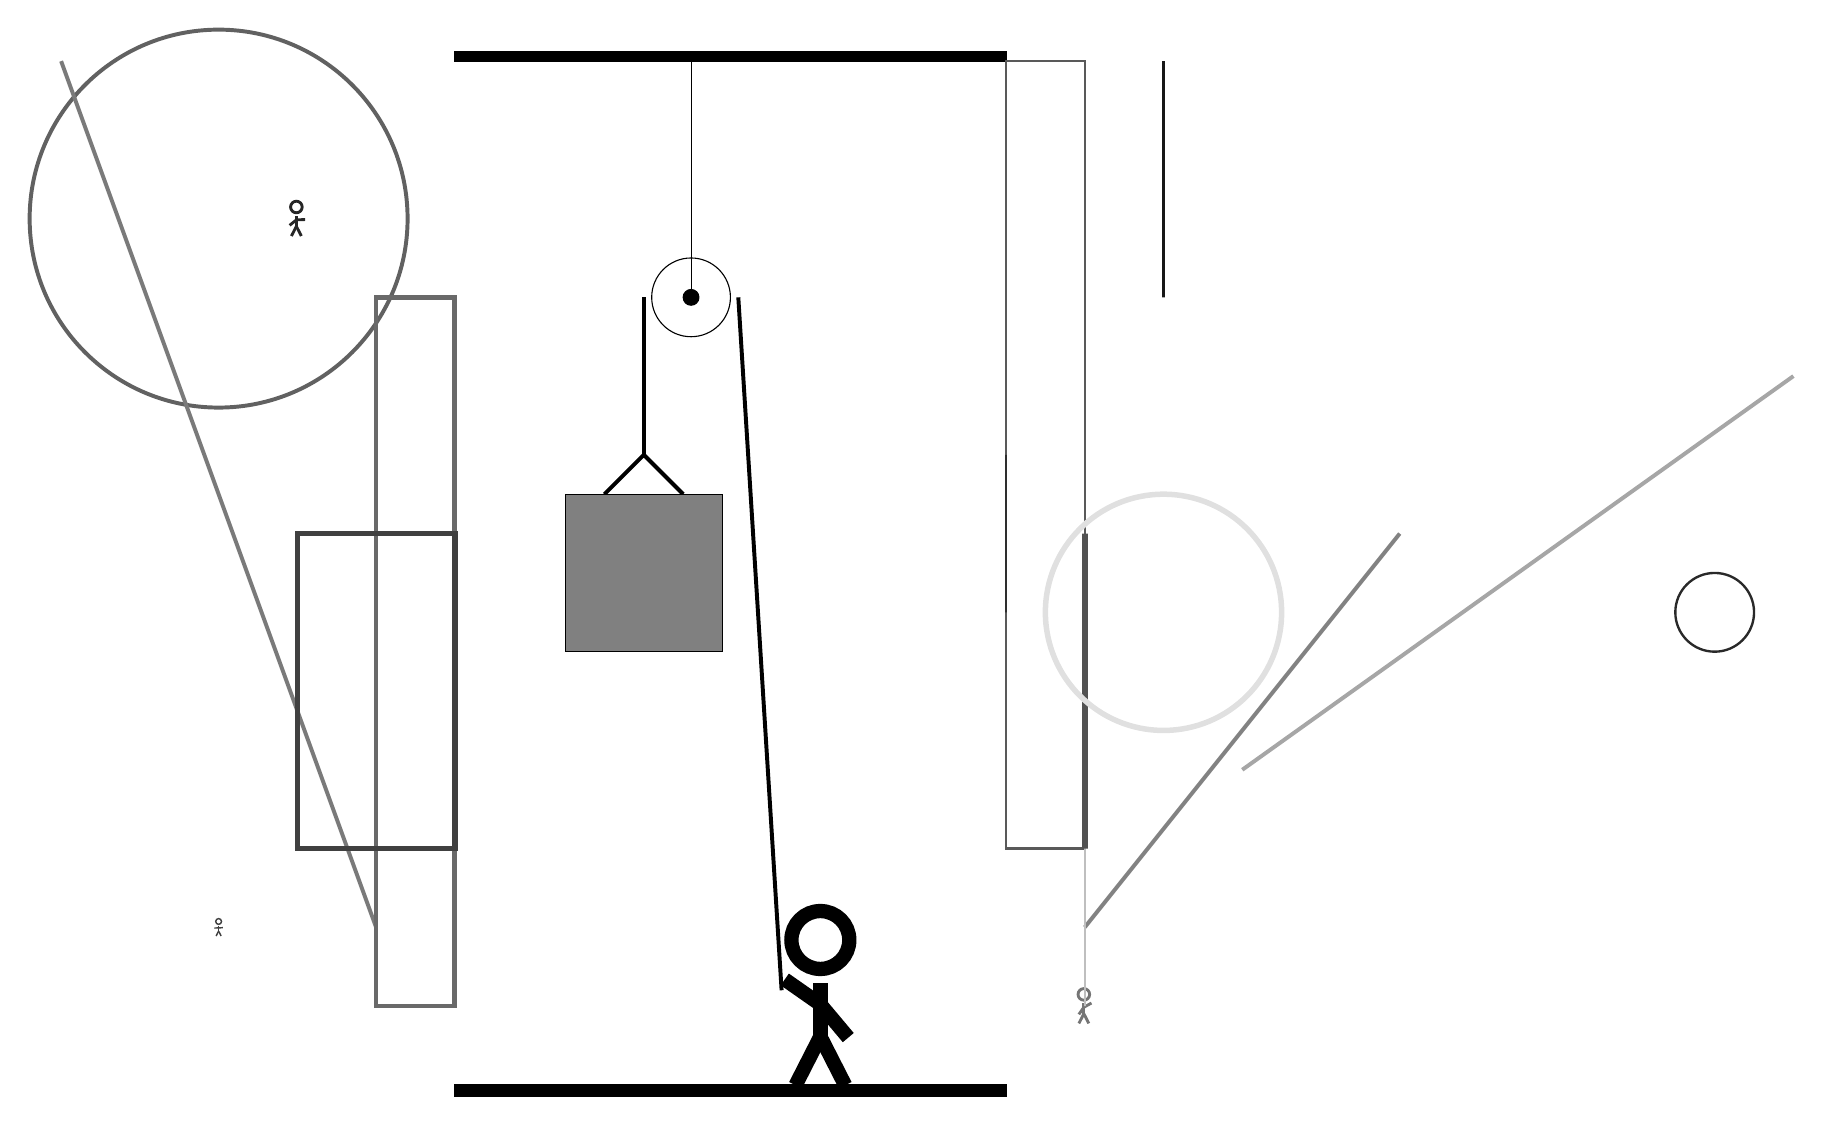
\begin{tikzpicture}
		%%%%% START %%%%%
		
		\draw[fill=black] (-2, 10) rectangle (5, 10.125);
		
		\draw[line width=0.3mm, color=black!65] (5, 0) rectangle (6, 10);
		
		\draw[line width=0.3mm, color=black!82] (5, 5) rectangle (5, 3);
		\draw [line width=0.5mm, color=black!62](-5, 8) circle (2.4);
		\draw[line width=0.7mm, color=black!68] (6, 4) rectangle (6, 0);
		\draw[line width=0.5mm, color=black!52](-3, -1) -- (-7, 10);
		\node[line width=0.6mm, color=black!85] at (-4, 8) {\Strichmaxerl[2][39][2]};
		\draw [line width=0.3mm, color=black!84](14, 3) circle (0.5);
		\node[line width=0.6mm, color=black!54] at (6, -2) {\Strichmaxerl[2][55][29]};
		\draw[line width=0.5mm, color=black!91] (7, 7) rectangle (7, 10);
		
		\draw [line width=0.7mm, color=black!12](7, 3) circle (1.5);
		
		\draw[line width=0.5mm, color=black!49](6, -1) -- (10, 4);
		\node[line width=0.3mm, color=black!75] at (-5, -1) {\Strichmaxerl[1][2][3]};
		\draw[line width=0.5mm, color=black!35](8, 1) -- (15, 6);
		
		\draw[line width=0.6mm, color=black!59] (-3, 7) rectangle (-2, -2);
		\draw[line width=0.7mm, color=black!75] (-2, 4) rectangle (-4, 0);
		\draw[line width=0.2mm, color=black!25] (6, 0) rectangle (6, -2);
		
		
		\draw (1, 7) circle (0.5);
		\draw[fill=black] (1, 7) circle (0.1);
		\draw (1, 10) -- (1, 7);
		
		\draw[line width=0.5mm] (-0.1, 4.5) -- (0.4, 5.0) -- (0.9, 4.5);
		\draw[fill=black!50] (-0.6, 4.5) rectangle (1.4, 2.5);
		
		\draw[line width=0.5mm] (0.4, 7) -- (0.4, 5.0);
		\centerarc[line width=0.5mm](1, 7)(0:180:0.6);
		\draw[line width=0.5mm](1.6, 7) -- (2.15, -1.8);
		
		\node at (2.6, -1.9) {\Strichmaxerl[10][-35][-50]};
		
		\draw[fill=black] (-2, -3) rectangle (5, -3.15);
		
		%%%%% END %%%%%
	\end{tikzpicture}
\end{document}